\documentclass[]{article}
\usepackage{lmodern}
\usepackage{amssymb,amsmath}
\usepackage{ifxetex,ifluatex}
\usepackage{fixltx2e} % provides \textsubscript
\ifnum 0\ifxetex 1\fi\ifluatex 1\fi=0 % if pdftex
  \usepackage[T1]{fontenc}
  \usepackage[utf8]{inputenc}
\else % if luatex or xelatex
  \ifxetex
    \usepackage{mathspec}
  \else
    \usepackage{fontspec}
  \fi
  \defaultfontfeatures{Ligatures=TeX,Scale=MatchLowercase}
\fi
% use upquote if available, for straight quotes in verbatim environments
\IfFileExists{upquote.sty}{\usepackage{upquote}}{}
% use microtype if available
\IfFileExists{microtype.sty}{%
\usepackage{microtype}
\UseMicrotypeSet[protrusion]{basicmath} % disable protrusion for tt fonts
}{}
\usepackage[margin=1in]{geometry}
\usepackage{hyperref}
\hypersetup{unicode=true,
            pdftitle={Untitled},
            pdfauthor={Jack Yan},
            pdfborder={0 0 0},
            breaklinks=true}
\urlstyle{same}  % don't use monospace font for urls
\usepackage{color}
\usepackage{fancyvrb}
\newcommand{\VerbBar}{|}
\newcommand{\VERB}{\Verb[commandchars=\\\{\}]}
\DefineVerbatimEnvironment{Highlighting}{Verbatim}{commandchars=\\\{\}}
% Add ',fontsize=\small' for more characters per line
\usepackage{framed}
\definecolor{shadecolor}{RGB}{248,248,248}
\newenvironment{Shaded}{\begin{snugshade}}{\end{snugshade}}
\newcommand{\KeywordTok}[1]{\textcolor[rgb]{0.13,0.29,0.53}{\textbf{#1}}}
\newcommand{\DataTypeTok}[1]{\textcolor[rgb]{0.13,0.29,0.53}{#1}}
\newcommand{\DecValTok}[1]{\textcolor[rgb]{0.00,0.00,0.81}{#1}}
\newcommand{\BaseNTok}[1]{\textcolor[rgb]{0.00,0.00,0.81}{#1}}
\newcommand{\FloatTok}[1]{\textcolor[rgb]{0.00,0.00,0.81}{#1}}
\newcommand{\ConstantTok}[1]{\textcolor[rgb]{0.00,0.00,0.00}{#1}}
\newcommand{\CharTok}[1]{\textcolor[rgb]{0.31,0.60,0.02}{#1}}
\newcommand{\SpecialCharTok}[1]{\textcolor[rgb]{0.00,0.00,0.00}{#1}}
\newcommand{\StringTok}[1]{\textcolor[rgb]{0.31,0.60,0.02}{#1}}
\newcommand{\VerbatimStringTok}[1]{\textcolor[rgb]{0.31,0.60,0.02}{#1}}
\newcommand{\SpecialStringTok}[1]{\textcolor[rgb]{0.31,0.60,0.02}{#1}}
\newcommand{\ImportTok}[1]{#1}
\newcommand{\CommentTok}[1]{\textcolor[rgb]{0.56,0.35,0.01}{\textit{#1}}}
\newcommand{\DocumentationTok}[1]{\textcolor[rgb]{0.56,0.35,0.01}{\textbf{\textit{#1}}}}
\newcommand{\AnnotationTok}[1]{\textcolor[rgb]{0.56,0.35,0.01}{\textbf{\textit{#1}}}}
\newcommand{\CommentVarTok}[1]{\textcolor[rgb]{0.56,0.35,0.01}{\textbf{\textit{#1}}}}
\newcommand{\OtherTok}[1]{\textcolor[rgb]{0.56,0.35,0.01}{#1}}
\newcommand{\FunctionTok}[1]{\textcolor[rgb]{0.00,0.00,0.00}{#1}}
\newcommand{\VariableTok}[1]{\textcolor[rgb]{0.00,0.00,0.00}{#1}}
\newcommand{\ControlFlowTok}[1]{\textcolor[rgb]{0.13,0.29,0.53}{\textbf{#1}}}
\newcommand{\OperatorTok}[1]{\textcolor[rgb]{0.81,0.36,0.00}{\textbf{#1}}}
\newcommand{\BuiltInTok}[1]{#1}
\newcommand{\ExtensionTok}[1]{#1}
\newcommand{\PreprocessorTok}[1]{\textcolor[rgb]{0.56,0.35,0.01}{\textit{#1}}}
\newcommand{\AttributeTok}[1]{\textcolor[rgb]{0.77,0.63,0.00}{#1}}
\newcommand{\RegionMarkerTok}[1]{#1}
\newcommand{\InformationTok}[1]{\textcolor[rgb]{0.56,0.35,0.01}{\textbf{\textit{#1}}}}
\newcommand{\WarningTok}[1]{\textcolor[rgb]{0.56,0.35,0.01}{\textbf{\textit{#1}}}}
\newcommand{\AlertTok}[1]{\textcolor[rgb]{0.94,0.16,0.16}{#1}}
\newcommand{\ErrorTok}[1]{\textcolor[rgb]{0.64,0.00,0.00}{\textbf{#1}}}
\newcommand{\NormalTok}[1]{#1}
\usepackage{graphicx,grffile}
\makeatletter
\def\maxwidth{\ifdim\Gin@nat@width>\linewidth\linewidth\else\Gin@nat@width\fi}
\def\maxheight{\ifdim\Gin@nat@height>\textheight\textheight\else\Gin@nat@height\fi}
\makeatother
% Scale images if necessary, so that they will not overflow the page
% margins by default, and it is still possible to overwrite the defaults
% using explicit options in \includegraphics[width, height, ...]{}
\setkeys{Gin}{width=\maxwidth,height=\maxheight,keepaspectratio}
\IfFileExists{parskip.sty}{%
\usepackage{parskip}
}{% else
\setlength{\parindent}{0pt}
\setlength{\parskip}{6pt plus 2pt minus 1pt}
}
\setlength{\emergencystretch}{3em}  % prevent overfull lines
\providecommand{\tightlist}{%
  \setlength{\itemsep}{0pt}\setlength{\parskip}{0pt}}
\setcounter{secnumdepth}{0}
% Redefines (sub)paragraphs to behave more like sections
\ifx\paragraph\undefined\else
\let\oldparagraph\paragraph
\renewcommand{\paragraph}[1]{\oldparagraph{#1}\mbox{}}
\fi
\ifx\subparagraph\undefined\else
\let\oldsubparagraph\subparagraph
\renewcommand{\subparagraph}[1]{\oldsubparagraph{#1}\mbox{}}
\fi

%%% Use protect on footnotes to avoid problems with footnotes in titles
\let\rmarkdownfootnote\footnote%
\def\footnote{\protect\rmarkdownfootnote}

%%% Change title format to be more compact
\usepackage{titling}

% Create subtitle command for use in maketitle
\newcommand{\subtitle}[1]{
  \posttitle{
    \begin{center}\large#1\end{center}
    }
}

\setlength{\droptitle}{-2em}

  \title{Untitled}
    \pretitle{\vspace{\droptitle}\centering\huge}
  \posttitle{\par}
    \author{Jack Yan}
    \preauthor{\centering\large\emph}
  \postauthor{\par}
      \predate{\centering\large\emph}
  \postdate{\par}
    \date{4/15/2019}


\begin{document}
\maketitle

\begin{Shaded}
\begin{Highlighting}[]
\CommentTok{# Import data}
\NormalTok{polite_df <-}\StringTok{ }
\StringTok{  }\KeywordTok{read_csv}\NormalTok{(}\StringTok{'./hw7/HW7-politeness_data.csv'}\NormalTok{) }\OperatorTok
\StringTok{  }\KeywordTok{as.tibble}\NormalTok{() }\OperatorTok\StringTok{ }\NormalTok{janitor}\OperatorTok{::}\KeywordTok{clean_names}\NormalTok{() }
\end{Highlighting}
\end{Shaded}

\paragraph{1. Exploratory Analysis}\label{exploratory-analysis}

Provide boxplots to show the relation between gender/attitude and pitch.

\begin{Shaded}
\begin{Highlighting}[]
\CommentTok{# boxplots }
\NormalTok{polite_df }\OperatorTok
\StringTok{  }\KeywordTok{ggplot}\NormalTok{(}\KeywordTok{aes}\NormalTok{(}\DataTypeTok{x =}\NormalTok{ gender, }\DataTypeTok{y =}\NormalTok{ frequency, }\DataTypeTok{color =}\NormalTok{ attitude)) }\OperatorTok{+}
\StringTok{    }\KeywordTok{geom_boxplot}\NormalTok{() }\OperatorTok{+}
\StringTok{    }\KeywordTok{theme_bw}\NormalTok{()}
\end{Highlighting}
\end{Shaded}

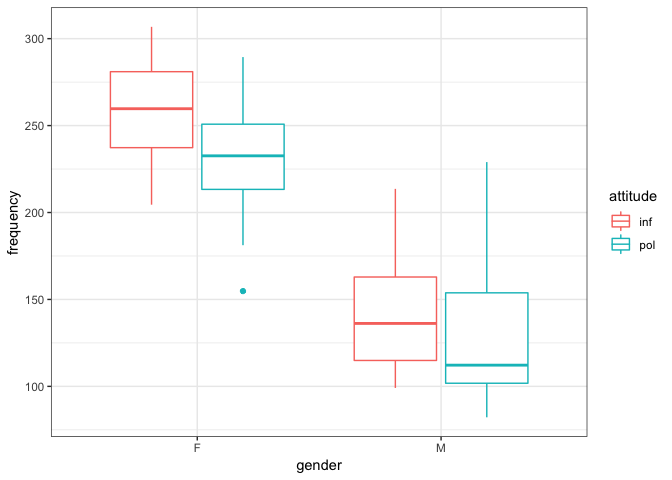
\includegraphics{Untitled_files/figure-latex/unnamed-chunk-2-1.pdf}

Males generally tend to have lower pitch than females. Within each
gender, informal attitude (inf) tends to have higher pitch than formal
attitude (pol).

\paragraph{2. Mixed Effects Model with Random
Intercept}\label{mixed-effects-model-with-random-intercept}

Fit a mixed effects model with random intercepts for different subjects
(gender and attitude being the fixed effects).

\begin{Shaded}
\begin{Highlighting}[]
\NormalTok{lmm =}\StringTok{ }\KeywordTok{lme}\NormalTok{(frequency }\OperatorTok{~}\StringTok{ }\NormalTok{gender }\OperatorTok{+}\StringTok{ }\NormalTok{attitude, }\DataTypeTok{random =} \OperatorTok{~}\DecValTok{1} \OperatorTok{|}\StringTok{ }\NormalTok{subject, }\DataTypeTok{method =} \StringTok{"REML"}\NormalTok{, }\DataTypeTok{data =}\NormalTok{ polite_df)}

\KeywordTok{VarCorr}\NormalTok{(lmm)}
\end{Highlighting}
\end{Shaded}

\begin{verbatim}
## subject = pdLogChol(1) 
##             Variance StdDev  
## (Intercept) 598.1953 24.45803
## Residual    847.7049 29.11537
\end{verbatim}

\begin{Shaded}
\begin{Highlighting}[]
\CommentTok{# var(Yi) = 598.1953 + 847.7049 = 1445.9}
\NormalTok{var =}\StringTok{ }\KeywordTok{as.numeric}\NormalTok{(}\KeywordTok{VarCorr}\NormalTok{(lmm)[[}\DecValTok{1}\NormalTok{]]) }\OperatorTok{+}\StringTok{ }\KeywordTok{as.numeric}\NormalTok{(}\KeywordTok{VarCorr}\NormalTok{(lmm)[[}\DecValTok{2}\NormalTok{]]); var }
\end{Highlighting}
\end{Shaded}

\begin{verbatim}
## [1] 1445.9
\end{verbatim}

\begin{Shaded}
\begin{Highlighting}[]
\CommentTok{# cov(Yij,Yik) = 598.2}
\NormalTok{cov =}\StringTok{ }\KeywordTok{as.numeric}\NormalTok{(}\KeywordTok{VarCorr}\NormalTok{(lmm)[[}\DecValTok{1}\NormalTok{]]); cov }
\end{Highlighting}
\end{Shaded}

\begin{verbatim}
## [1] 598.1953
\end{verbatim}

The covariance matrix for a subject \(Y_i\) follows a compound symmetry
pattern with \(var(Y_{ij})=1445.9\) and \(cov(Y_{ij},Y_{ik})=598.2\).
There are 14 measurements within each subject, so the covariance matrix
is a 14*14 matrix with \(var(Y_{ij})=1445.9\) as diagonal values and
\(cov(Y_{ij},Y_{ik})=598.2\) as off-diagonal values.

\(var(Y_{i})=\begin{bmatrix}  1445.9 & 598.2 & \dots & 598.2 \\  598.2 & 1445.9 & \\  \vdots & &\ddots & \vdots\\  598.2 & & \dots & 1445.9  \end{bmatrix}_{14 \times 14}\)

\begin{Shaded}
\begin{Highlighting}[]
\CommentTok{# covariance matrix for the REML estimates of fixed effects}
\KeywordTok{vcov}\NormalTok{(lmm)}
\end{Highlighting}
\end{Shaded}

\begin{verbatim}
##             (Intercept)       genderM   attitudepol
## (Intercept)   229.67362 -2.195819e+02 -2.018345e+01
## genderM      -219.58189  4.391638e+02  6.451438e-15
## attitudepol   -20.18345  6.451438e-15  4.036690e+01
\end{verbatim}

\begin{Shaded}
\begin{Highlighting}[]
\CommentTok{# BLUPs for subject-speci􏰍c intercepts}
\KeywordTok{random.effects}\NormalTok{(lmm)}
\end{Highlighting}
\end{Shaded}

\begin{verbatim}
##    (Intercept)
## F1  -13.575831
## F2   10.170522
## F3    3.405309
## M3   27.960288
## M4    4.739325
## M7  -32.699613
\end{verbatim}


\end{document}
